\subsubsection{Foldy-Wouthuysen contribution to $\alpha_E$ at $m_\pi$= 357 MeV.}
In order to extract the lattice measurement of the neutron's electric polarizability,
one has to calculate the point-like contribution present in its energy spectrum. Such a 
a contribution to dipole electric polarizability is long-know~\cite{foldy}. There are ten
leading Foldy contributions for a zero-momentum neutron, which were determined
from a Foldy-Wouthuysen transformation constructed in such a form as to yield
the energy shift of a neutron in the presence of an external electromagnetic field.
These contributions are reported in~\cite{foldywouthuysen}, and the Foldy-Wouthuysen
electric polarizability contribution $\alpha_{\text{FW}}$ is
\begin{equation}
\alpha_{\text{FW}}=-\frac{-\mu^2}{m_n}
\label{fwcontrib}
\end{equation}
where $\mu$ is the anomalous magnetic moment of the neutron and $m_n$ is the 
neutron mass. Given that the lattice measurements of the electric polarizability are
conducted at $m_\pi=$ 357 MeV, the point-like contribution~\ref{fwcontrib} has to be
evaluated at te pion mass scale. For example, in~\cite{engelhardt4}, the isovector and
isoscalar normalized anomalous magnetic moments are given for the nucleon at 
$m_\pi=$ 355 MeV, which is very close to our working pions mass of 357 MeV. These are,
respectively, $\kappa_v^{\text{norm}}=2.518(57)$ and $\kappa_s^{\text{norm}}=-0.030(22)$
in magnetons. The neutron anomalous magnetic moment is given by
\begin{equation}
\kappa=\frac{\kappa_s^{\text{norm}}-\kappa_v^{\text{norm}}}{2}=-1.274\pm0.031
\end{equation}
As a function of the neutron mass $m_n$, the magnetic moment in GeV$^{-1}$ is
\begin{equation}
\mu=\kappa\sqrt{\frac{1}{137}}\frac{1}{2m_n^{\text{phys}}}
\label{anomalous}
\end{equation}
Evaluating~\ref{anomalous} at the physical neutron mass $m_n^{\text{phys}}$, as given 
in~\cite{PDG2017}, the magnetic moment is then
\begin{equation}
\mu_{357\text{ MeV}}=-0.05792\pm0.0014\text{ GeV}^{-1}
\label{magmom}
\end{equation}
On the other hand, at $m_\pi=355.98(80)$ MeV the neutron mass is $m_n=1154.8(80)$ 
MeV, as given in~\cite{bratt}. This mass value, along with the result given in~\ref{magmom}, lead to 
a Foldy-Wouthuysen contribution (c.f.~\ref{fwcontrib})
\begin{equation}
\alpha_{\text{FW}}^{357\text{ MeV}}=(-0.2232\pm7.7\times 10^{-7})\text{ }10^{-4}\text{ fm}^{-3}
\end{equation}
As detailed in~\cite{foldywouthuysen},~\ref{fwcontrib} results from the energy shift of a 
pointlike neutron, so it must be subtracted from the $\alpha_E$ obtained from the lattice 
measurements described in this work.
%%%%%%%%%%%%%%%%%%%%%%%%%%%
%%%%%%%%%%%%%%%%%%%%%%%%%%%
\subsubsection{Electric polarizability $\alpha_E$, $m_{\pi}$=357 MeV measurements for
conected diagrams in the 3-window analysis}
\label{357}
Several data sets were used in our analysis; these are labeled as \textcolor{red}{\textit{original}},
in which the diagrams involve smeared sinks, \textcolor{red}{\textit{points}}, in which
the neutron sink is point-like,  \textcolor{red}{\textit{multi}}, which has increased statistics
in the denominator that defines de correlator ratio $R_2(t)$, and  
\textcolor{red}{\textit{multi point}}, which refers to the dataset with point-like neutron
sinks and improved statistics.In the analysis of these data sets, a technicality 
has been identified in~\cite{engelhardt1};a time-independent Hamiltonian ensures 
a stationary neutron wave function, while a time dependence is introduced by 
the smeared neutron sink, which would have to be addressed by considering 
additional contributions from other diagrams than those shown in \ref{fig:diagrams}. 
These additional diagram contributions have not been evaluated in this work. 
Our \textcolor{red}{point} and \textcolor{red}{multi point} datasets avoid the 
aforementioned systematic effects; a point neutron sink is time-independent 
and invariant under gauge transformations of the external field. For the previous reasons,
the preferred data set in this work is the one with point neutron sinks 
and improved denominator statistics.

The slopes presented in this work were obtained by performing $\chi^2$ 
fits to the $R_2(t)$ data for a range of choice $5a\le t\le7a$ in the three-window analysis,
in which linear functions are fitted for the selected range at the three time windows
of the cubic correlator ratio. The slopes obtained from these fits are three points in
a quadratic function, which represents the derivative of the cubic, for which the
extremal value is determined. \textcolor{red}{This extremal values were corrected for curvature of the
fitted function}. This work also considers the fitting ranges $4a\le t\le 8a$ and $3a\le t\le 9a$ 
as alternatives. Tables~\ref{Table:ConnectedMultipoint}, \ref{Table:ConnectedPoint},
 \ref{Table:ConnectedMulti} summarize our results.
 
 The static electric polarizability for the three fitting ranges are presented 
 in~\ref{Tab:ConnectedPolarizabilities} for the \textcolor{red} {``Multi point" dataset}, 
 with and without the Foldy-Wouthuysen contribution~\cite{foldywouthuysen}. 
 The electric polarizability measurements are consistent with the reported in~\cite{engelhardt2}. 
 Similar result were obtained for the \textcolor{red}{``Multi" and ``Point" datasets}, these are
 show in tables~\ref{Tab:ConnectedPolarizabilitiesMulti}, \ref{Tab:ConnectedPolarizabilitiesPoint}.
 
 %%%%%3-window Connected EXTREMUM TABLE%%%%%%
\begin{table}
\begin{center}
    \begin{tabular}{ | l | p{2.2cm} | p{2.2cm} | p{2.2cm} |}
    \hline
     Fit & 5 to 7   &4 to 8   & 3 to 9  \\ \hline
     Extremal (in $a^3$)&  -0.0126966 $\pm$ 0.00767283  &  -0.0149389 $\pm$ 0.00576662  & -0.0193804 $\pm$ 0.00422518  \\ \hline
     position ($t/a$)& 6.4303 $\pm$ 0.244647  & 6.74468 $\pm$ 0.186373   &  7.27915 $\pm$ 0.133938   \\ \hline
    \end{tabular}
\end{center}
\caption{\textcolor{red}{``Multi point"} Extremal values and their positions for the $\chi^2$ linear fits in the 3-window analysis with parabola minimum lift \textcolor{red}{correction} and for connected diagrams.}
\label{Table:ConnectedMultipoint}
\end{table}

%%%%%Point EXTREMUM TABLE%%%%%%
%%%%%POINT Connected EXTREMUM TABLE%%%%%%
\begin{table}
\begin{center}
    \begin{tabular}{ | l | p{2.2cm} | p{2.2cm} | p{2.2cm} |}
    \hline
     Fit & 5 to 7   &4 to 8   & 3 to 9  \\ \hline
     Extremal (in $a^3$)&   -0.0150773 $\pm$ 0.0078205   &   -0.015437 $\pm$ 0.00585418   &  -0.0185265 $\pm$ 0.00433289   \\ \hline
     position ($t/a$)&  6.27146 $\pm$ 0.269647  &  6.58599 $\pm$ 0.199774    &  7.14987 $\pm$ 0.139975    \\ \hline
    \end{tabular}
\end{center}
\caption{\textcolor{red}{``Point" Extremal} values and their positions for the $\chi^2$ linear fits in the 3-window analysis with parabola minimum lift \textcolor{red}{correction} and for connected diagrams.}
\label{Table:ConnectedPoint}
\end{table}

%%%%%MULTI Connected EXTREMUM TABLE%%%%%%
\begin{table}
\begin{center}
    \begin{tabular}{ | l | p{2.2cm} | p{2.2cm} | p{2.2cm} |}
    \hline
     Fit & 5 to 7   &4 to 8   & 3 to 9  \\ \hline
     Extremal (in $a^3$)&   -0.00585051 $\pm$ 0.00771231   &  -0.00850892 $\pm$ 0.0684786   &  -0.00898652 $\pm$ 0.00483103   \\ \hline
     position ($t/a$)&  7.69036 $\pm$ 0.268354   &  7.89946 $\pm$ 1.68311   &   8.21679 $\pm$ 0.174493    \\ \hline
    \end{tabular}
\end{center}
\caption{\textcolor{red}{``Multi"} Extremal values and their positions for the $\chi^2$ linear fits in the 3-window analysis with parabola minimum lift \textcolor{red}{correction} and for connected diagrams}
\label{Table:ConnectedMulti}
\end{table}
%%%%%%%%%%%%%%%%%%%%%%%%%%
%%%%%%%%Slope figures%%%%%%%%%%%
\begin{figure}[h!]
\centering
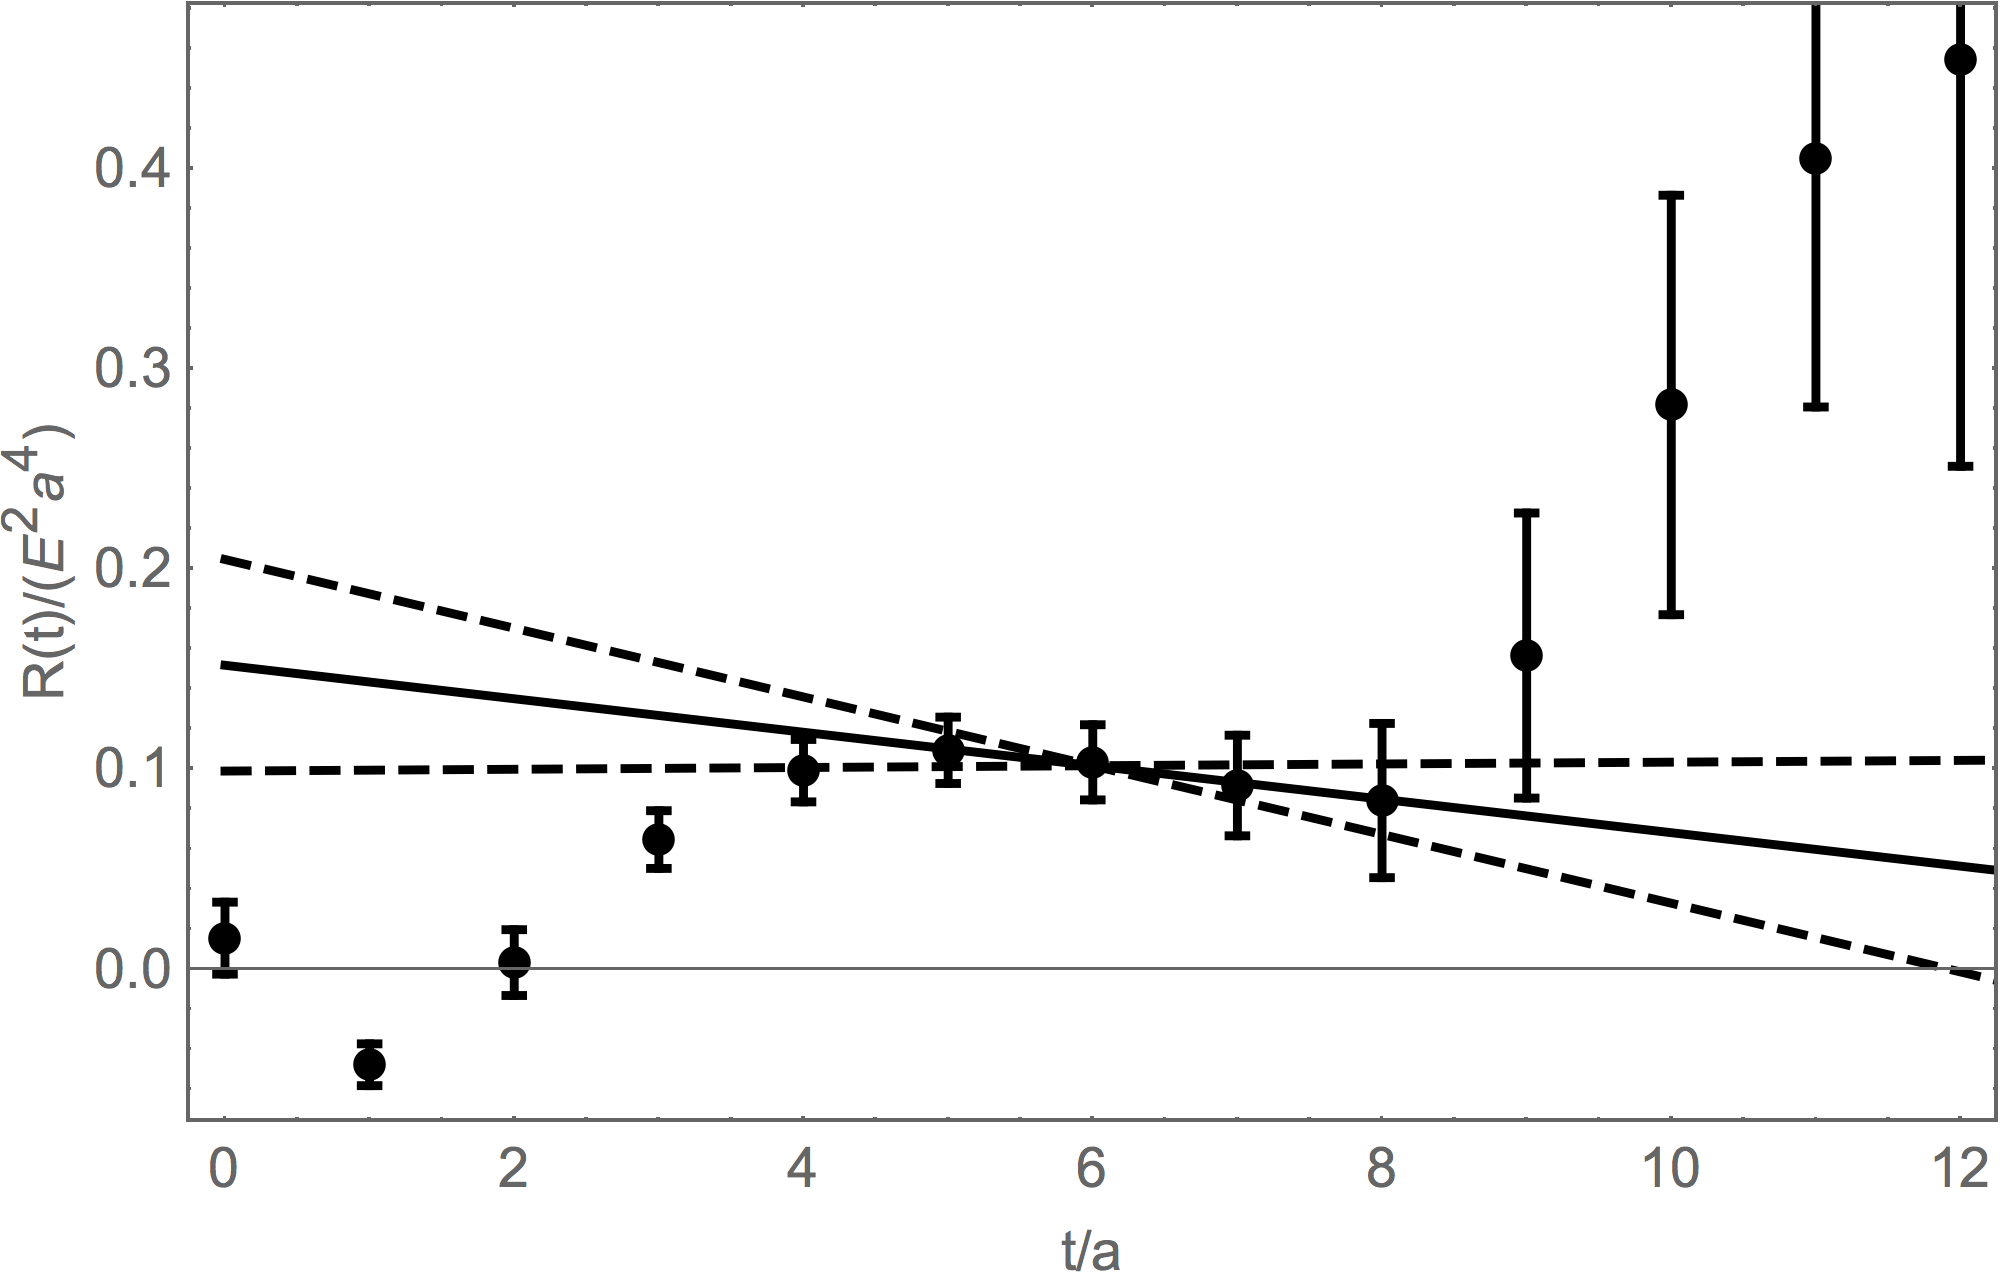
\includegraphics[width=5cm]{figures/shshLineCS.png}
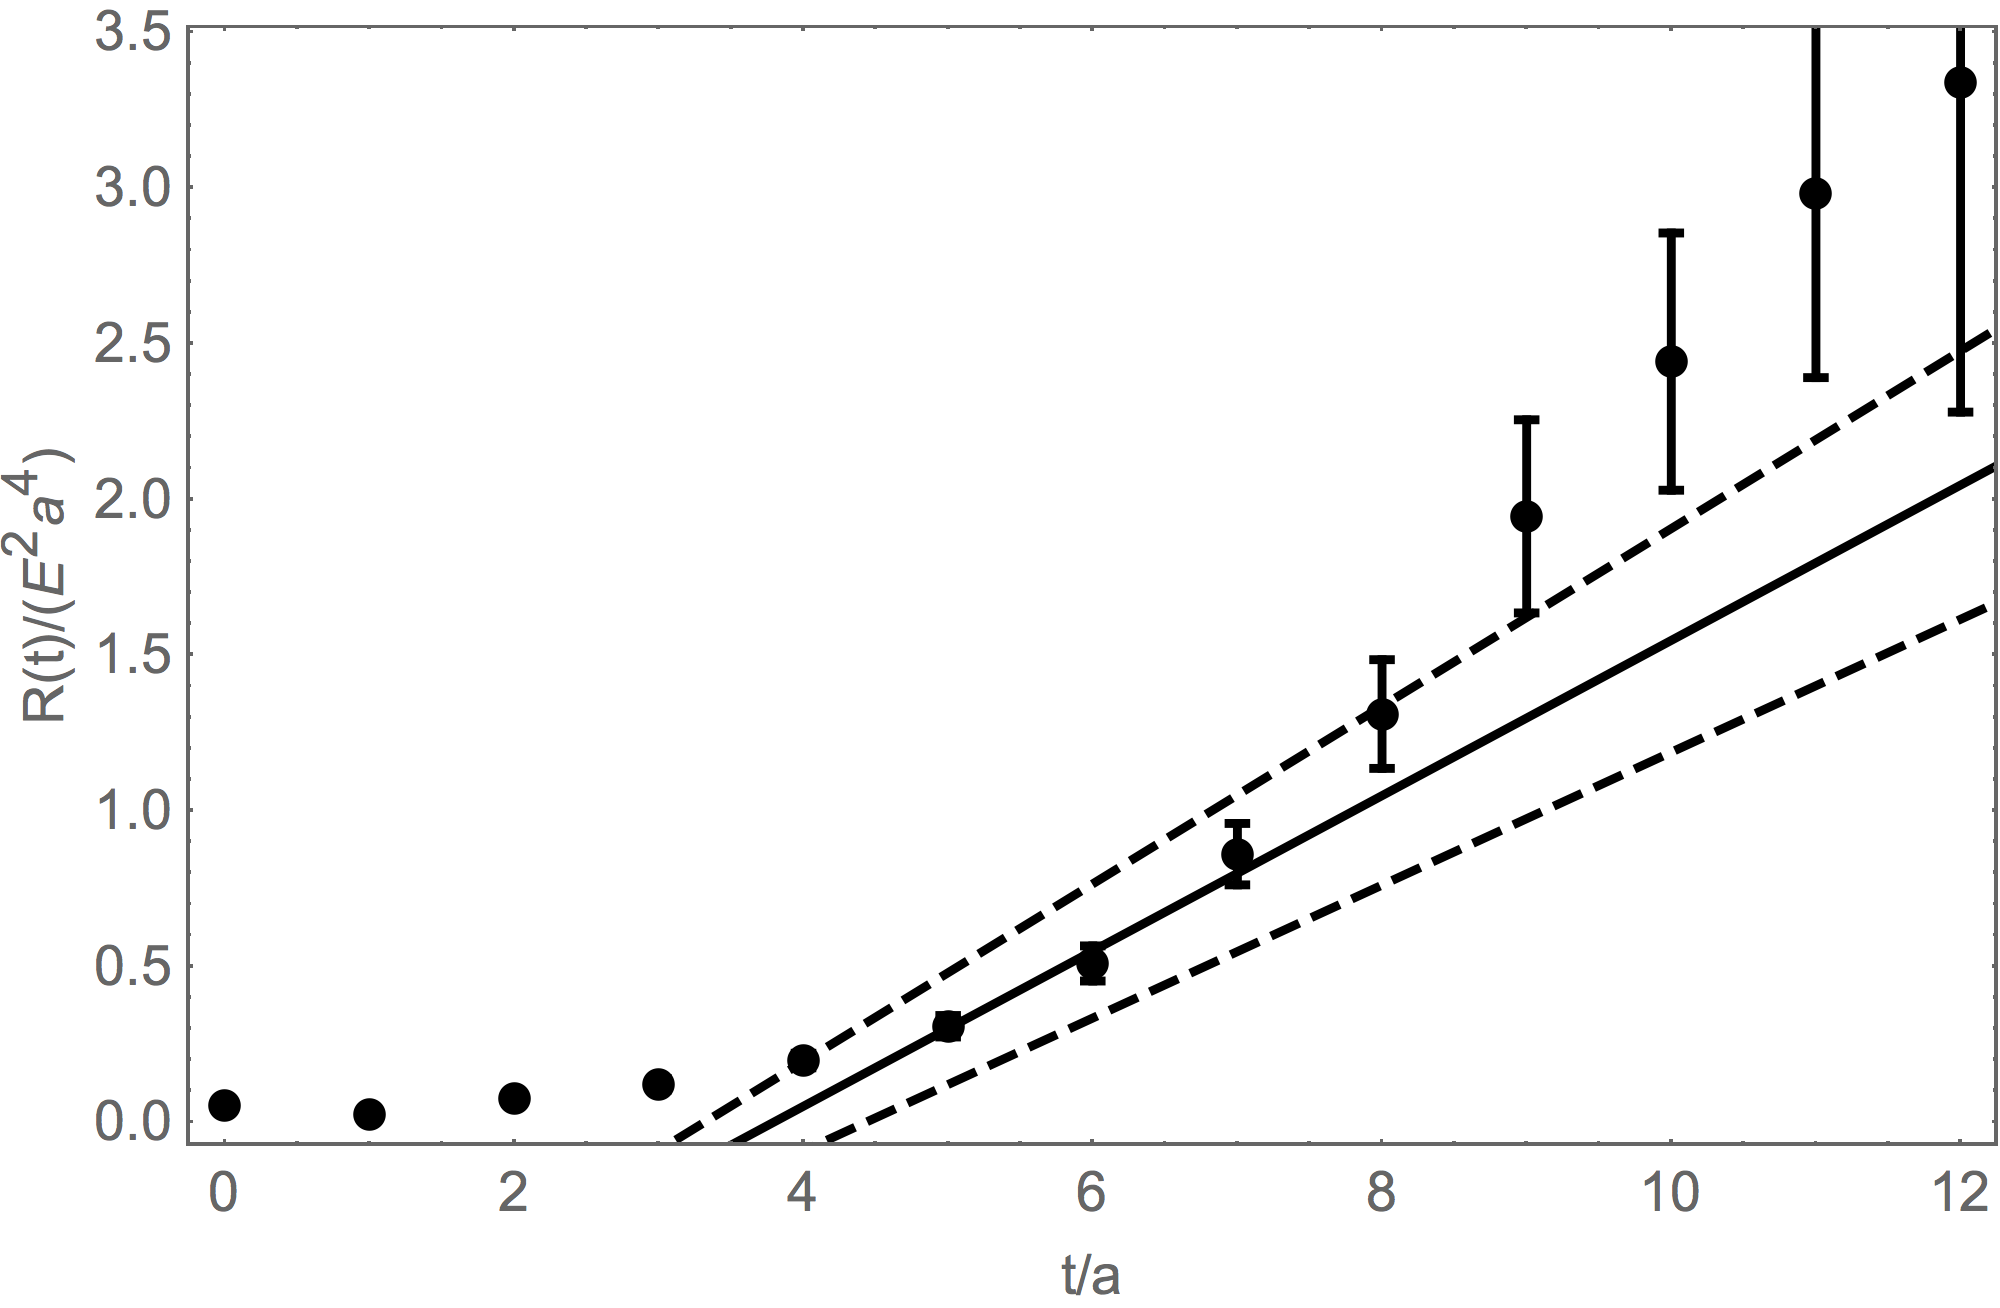
\includegraphics[width=5cm]{figures/from0LineCS.png}
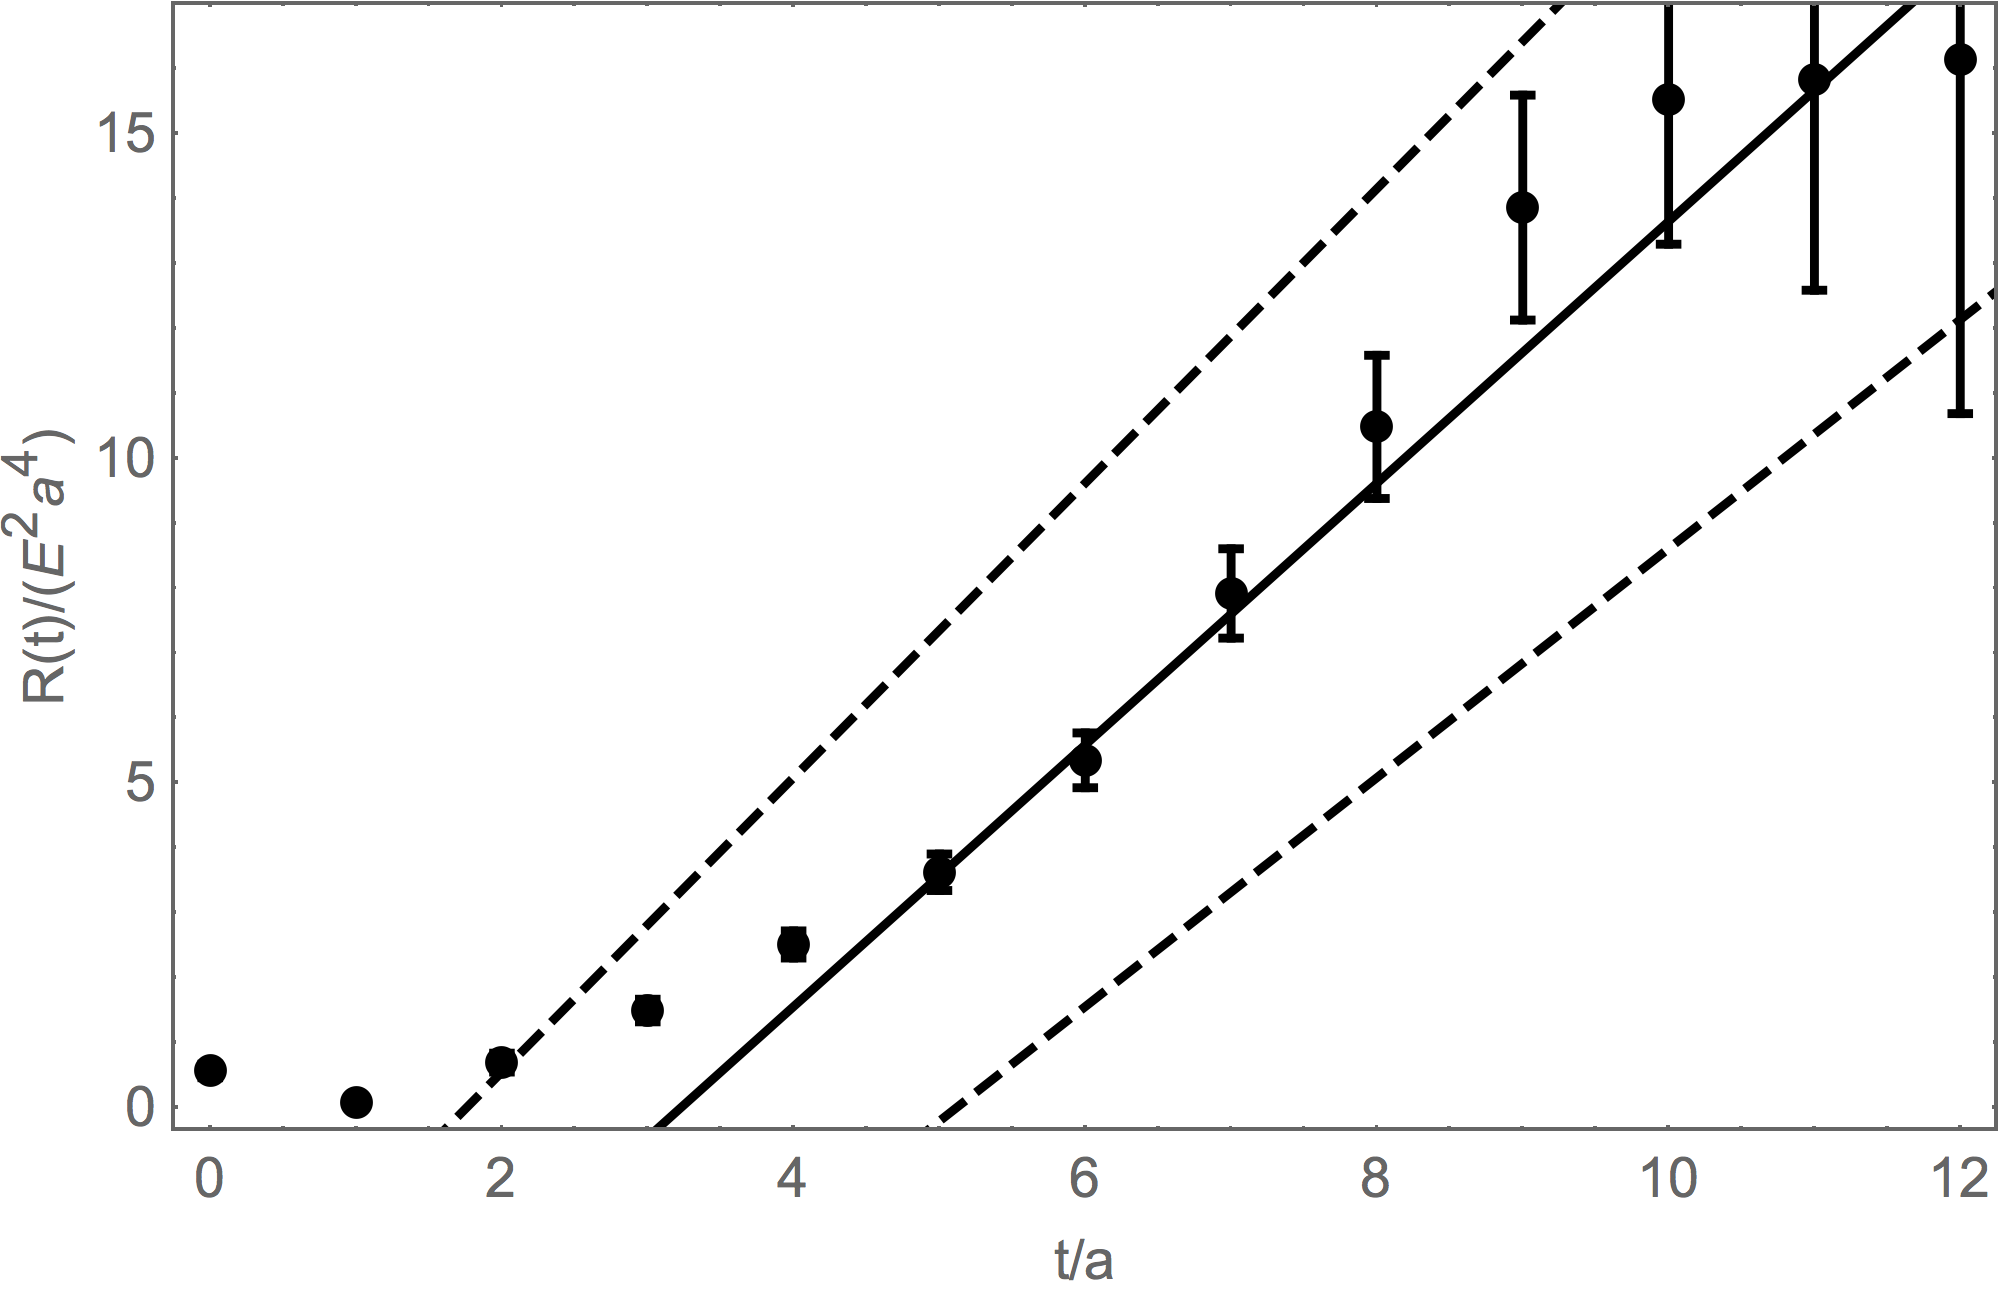
\includegraphics[width=5cm]{figures/shortLineCS.png}\\
\caption{Correlator ratio $R(t)$ for the connected diagrams a), b), f), shown in Fig.~\ref{fig:diagrams}, in units of $E^2a^4$. In these plots, the neutron source was placed at the fixed location $t=0$, and the background field, c.f.~\ref{gauge}, was varied with $t_0=6a$, $t_0=0$, $t_0=-10a$ (from left to right). The dashed lines delimit the linear fit uncertainty in the slope.}
\label{fig: alphaconnected}
\end{figure}
%%%%%%%%%%%%%%%%%%%%%%%%%%%%%

%%%%%%%%%Electric Polarizability Results%%%%%
%%%%%%%%%%Multi point Polarizability 10^-4 fm^3%%%%%%
\begin{table}[h!]
\begin{center}
    \begin{tabular}{ | p{2cm}  | p{4cm} | p{4cm} | }
    \hline
     Fitting range ($t/a$) & $\alpha_E$ ($10^{-4}$ $\text{fm}^3$)    & $\alpha_E-\alpha_{FW}$ ($10^{-4}$ $\text{fm}^3$)       \\ 
     \hline
     5 to 7 & 0.484154 $\pm$ 0.292584      &    0.707351$\pm$ 0.292584          \\ \hline
     4 to 8 &  0.569657 $\pm$ 0.219895       &  0.792854 $\pm$ 0.219895             \\ \hline
     3 to 9 &    0.739023 $\pm$ 0.161117       &  0.96222 $\pm$ 0.161117            \\ \hline
    \end{tabular}
\end{center}
\caption{Static electric polarizability  $\alpha_E$ and static electric polarizability minus Foldy-Wouthuysen contribution $\alpha_E-\alpha_{FW}$ from the extremal values (connected diagrams, $\chi^2$ fits, \textcolor{red}{``multi point"} dataset) of the three fitting ranges in units of $10^{-4}$ $\text{fm}^3$.}
\label{Tab:ConnectedPolarizabilities}
\end{table}

%%%%%%%%%%Multi Polarizability 10^-4 fm^3%%%%%%
\begin{table}
\begin{center}
    \begin{tabular}{ | p{2cm}  | p{4cm} | p{4cm} | }
    \hline
     Fitting range ($t/a$) & $\alpha_E$ ($10^{-4}$ $\text{fm}^3$)    & $\alpha_E-\alpha_{FW}$ ($10^{-4}$ $\text{fm}^3$)       \\ 
     \hline
     5 to 7 &    0.223094 $\pm$ 0.29409      &   0.446291 $\pm$ 0.29409           \\ \hline
     4 to 8 &   0.324466 $\pm$ 2.61126       &    0.547663 $\pm$ 2.61126          \\ \hline
     3 to 9 &   0.342678 $\pm$ 0.184219        &      0.565875 $\pm$ 0.184219         \\ \hline
    \end{tabular}
\end{center}
\caption{ Static electric polarizability  $\alpha_E$ and static electric polarizability minus Foldy-Wouthuysen contribution $\alpha_E-\alpha_{FW}$ from the extremal values (connected diagrams, $\chi^2$ fits, \textcolor{red}{``multi"} dataset) of the three fitting ranges in units of $10^{-4}$ $\text{fm}^3$.}
\label{Tab:ConnectedPolarizabilitiesMulti}
\end{table}
%%%%%%%%%%%%%%%%%%%%%%%%%%%%%
%%%%%%%%%%Point Polarizability 10^-4 fm^3%%%%%%
\begin{table}
\begin{center}
    \begin{tabular}{ | p{2cm}  | p{4cm} | p{4cm} | }
    \hline
     Fitting range ($t/a$) & $\alpha$ ($10^{-4}$ $\text{fm}^3$)    & $\alpha-\alpha_{FW}$ ($10^{-4}$ $\text{fm}^3$)       \\ 
     \hline
     5 to 7 &    0.574936 $\pm$ 0.298215      &   0.798132 $\pm$ 0.298215           \\ \hline
     4 to 8 &   0.588652 $\pm$ 0.223234       &    0.811848 $\pm$ 0.223234          \\ \hline
     3 to 9 &  0.706462 $\pm$ 0.165224        &     0.929658 $\pm$ 0.165224          \\ \hline
    \end{tabular}
\end{center}
\caption{Static electric polarizability  $\alpha_E$ and static electric polarizability minus Foldy-Wouthuysen contribution $\alpha_E-\alpha_{FW}$ from the extremal values (connected diagrams, $\chi^2$ fits, \textcolor{red}{``point"} dataset) of the three fitting ranges in units of $10^{-4}$ $\text{fm}^3$.}
\label{Tab:ConnectedPolarizabilitiesPoint}
\end{table}




